% =============================================================================
% Module 9: Strong Lensing by Galaxies: Applications
% =============================================================================
% Sources: Congdon & Keeton Ch. 6.5-6.6, Narayan & Bartelmann Sec. 3.6-3.7,
%          Saha et al. (2024), Schneider & Sluse (2014), Treu (2010),
%          Birrer et al. (2020), Wong et al. (2020)
% Mathematica: ../Mathematica/09_Galaxy_Lensing_Applications/
% =============================================================================

\chapter{Strong Lensing by Galaxies: Applications}
\label{ch:galaxy_lensing}

\begin{quote}
\textit{The Einstein radius is a most useful quantity to express the lensing strength
of an object, and it is usually very robustly determined via strong lens
models [\ldots].  As a consequence, the mass enclosed in the cylinder of radius
equal to the Einstein radius can be measured to within 1--2\%, including all
random and systematic uncertainties.}
\hfill --- T.~Treu, \textit{Ann.\ Rev.\ Astron.\ Astrophys.} \textbf{48}, 87 (2010)
\end{quote}

\noindent
In Modules~\ref{ch:axisymmetric_models} and~\ref{ch:elliptical_models}
we developed the theory and the lens models: the SIS, SIE, critical
curves, caustics, and image configurations.  These are the
\textit{tools}.  Now we apply them.

Galaxy-scale strong lensing is one of the most powerful techniques in
modern astrophysics.  It addresses fundamental questions:
\begin{itemize}[nosep]
    \item \textbf{What is the total mass of a galaxy?}  Lensing
          measures the projected mass within the Einstein radius,
          including dark matter.
    \item \textbf{How is mass distributed?}  Combining lensing with
          stellar kinematics constrains the density profile slope.
    \item \textbf{What is the expansion rate of the universe?}
          Time delays between multiple images, combined with a lens
          model, yield $\Hubble$ --- independent of the cosmic
          distance ladder.
    \item \textbf{What are the limits of what lensing can tell us?}
          Fundamental degeneracies --- most notably the
          \textit{mass-sheet degeneracy} --- limit the information
          that lensing alone can provide.
\end{itemize}

This module connects the lens modeling formalism to these real
astrophysical applications.  Understanding the degeneracies is as
important as understanding the models themselves.

\medskip
\noindent
\textbf{Companion Mathematica files:}
\begin{itemize}[nosep]
    \item \mathlink{09_Galaxy_Lensing_Applications/galaxy\_lensing.wl}{galaxy\_lensing.wl}
          --- mass from Einstein radius, mass-sheet degeneracy
          demonstration, power-law profile analysis, $\Hubble$ from
          time delays; figure generation for all module figures
    \item \mathlink{09_Galaxy_Lensing_Applications/mass\_sheet\_demo.nb}{mass\_sheet\_demo.nb}
          --- interactive notebook: MSD visualizer with slider for
          $\lambda$, power-law profile explorer, $\Hubble$ estimator
          from time delays
\end{itemize}


% =====================================================================
\section{Lens Modeling Overview}
\label{sec:lens_modeling_overview}

Before applying lensing to astrophysics, we must understand what goes
into building a lens model and what data constrain it.

\subsection{Parametric Models: SIE + External Shear}

The standard approach to modeling galaxy-scale strong lenses uses a
\textbf{parametric} mass model.  The workhorse is the singular
isothermal ellipsoid (SIE, Module~\ref{ch:elliptical_models}) plus
external shear:
\begin{equation}
    \kappab(\vectheta) = \frac{\thetaE\,\sqrt{q}}{
    2\sqrt{q^2\theta_1^2 + \theta_2^2}}
    \label{eq:sie_kappa_recap}
\end{equation}
with an external shear $\gamma_{\mathrm{ext}}$ at position angle
$\phi_\gamma$.  The model parameters are:
\begin{center}
\begin{tabular}{ll}
\toprule
\textbf{Parameter} & \textbf{Physical meaning} \\
\midrule
$\thetaE$ & Einstein radius (sets the mass scale) \\
$q$ & Axis ratio ($b/a$, sets the ellipticity) \\
$\theta_{1,c}$, $\theta_{2,c}$ & Lens center position \\
$\phi_q$ & Position angle of the mass distribution \\
$\gamma_{\mathrm{ext}}$ & External shear magnitude \\
$\phi_\gamma$ & External shear position angle \\
\bottomrule
\end{tabular}
\end{center}
This gives 7 lens parameters (or 5 if the center is fixed to the
observed galaxy light).  The source position $\vecbeta =
(\beta_1, \beta_2)$ adds 2 more unknowns, for a total of 9 (or 7)
free parameters.

\subsection{What Data Constrain the Model}

The observational constraints for a strong lens system are:
\begin{itemize}
    \item \textbf{Image positions:} Each image gives 2 constraints
          ($\theta_{1,i}$, $\theta_{2,i}$).  A quad system with 4
          images gives 8 constraints.
    \item \textbf{Flux ratios:} Each flux ratio gives 1 constraint
          (the ratio of magnifications).  Three independent flux ratios
          for a quad.
    \item \textbf{Time delays:} Each time delay gives 1 constraint.
          Three independent delays for a quad.
    \item \textbf{Extended arcs:} If the source is extended (a galaxy
          rather than a quasar), the arc morphology provides many more
          constraints (effectively constraining the lens potential on a
          grid).
\end{itemize}

\subsection{Degrees of Freedom}

For a quad lens modeled with SIE + shear:
\begin{itemize}
    \item Constraints from image positions alone: $4 \times 2 = 8$.
    \item Free parameters (with center fixed): 7.
    \item Degrees of freedom: $8 - 7 = 1$ (marginally constrained).
\end{itemize}
This is why quad lenses are so valuable: they provide just enough
constraints to determine the SIE + shear model from astrometry alone.
Double lenses ($2 \times 2 = 4$ constraints) are under-constrained
for SIE + shear.  Extended arcs provide many more constraints and can
support more complex models.

\subsection{Free-Form Models}

An alternative to parametric models is \textbf{free-form} or
\textbf{pixelated} modeling, where the lens potential is
reconstructed on a grid without assuming a specific functional form.
Programs like \texttt{PixeLens} (Saha \& Williams 2004) and
\texttt{GLASS} (Coles et al.\ 2014) take this approach.  Free-form
models are less biased by the assumed mass profile but have more
degrees of freedom and thus require regularization or priors.


% =====================================================================
\section{The Einstein Radius as a Mass Estimator}
\label{sec:einstein_mass}

\subsection{The Model-Independent Mass Measurement}

The single most important result in galaxy-scale strong lensing is
that the Einstein radius directly gives the enclosed projected mass.
For \textit{any} circularly symmetric lens, the projected mass
enclosed within the Einstein radius is (Congdon \& Keeton
eq.~7.9):
\begin{equation}
    \boxed{
    M(\le \thetaE) = \pi\,\thetaE^2\,\Dd^2\,\Sigmacr
    }
    \label{eq:mass_einstein}
\end{equation}

This follows from the definition of the Einstein radius as the
angular radius where $\kappab_{\mathrm{mean}} = 1$, i.e., where
the mean convergence within that radius equals unity.  Recall that
$\kappab = \Sigma/\Sigmacr$, so $\kappab_{\mathrm{mean}} = 1$
means the mean surface mass density within $\thetaE$ equals the
critical surface mass density.  The enclosed mass is then the
critical density times the area:
\begin{equation}
    M_{\mathrm{E}} = \Sigmacr \times \pi (\Dd\,\thetaE)^2
    = \pi\,\thetaE^2\,\Dd^2\,\Sigmacr \,.
    \label{eq:mass_einstein_derivation}
\end{equation}

The critical surface mass density is
(Module~\ref{ch:lens_equation}):
\begin{equation}
    \Sigmacr = \frac{\speedoflight^2}{4\pi \Gnewton}
    \,\frac{\Ds}{\Dd\,\Dds} \,.
    \label{eq:sigma_cr_recap}
\end{equation}
Substituting:
\begin{equation}
    \boxed{
    M_{\mathrm{E}} = \frac{\speedoflight^2}{4\Gnewton}
    \,\thetaE^2\,\frac{\Dd\,\Ds}{\Dds}
    }
    \label{eq:mass_from_thetaE}
\end{equation}

\begin{remark}
Equation~\eqref{eq:mass_from_thetaE} is \textbf{model-independent}
for any circularly symmetric lens.  It depends only on the observed
Einstein radius $\thetaE$ and the angular diameter distances
(which require knowing the redshifts $z_d$ and $z_s$ and adopting
a cosmology).  It does not depend on the radial mass profile.  This
is the great power of strong lensing as a mass measurement tool.
\end{remark}

\begin{derivation}[Substitution and a unit check]
\[
  \pi\thetaE^2\Dd^2\Sigmacr
  = \pi\thetaE^2\Dd^2\,\frac{\speedoflight^2}{4\pi\Gnewton}\frac{\Ds}{\Dd\Dds}
  = \frac{\speedoflight^2}{4\Gnewton}\,\thetaE^2\,\frac{\Dd\Ds}{\Dds}.
\]
Units: $[\speedoflight^2/\Gnewton] = (\mathrm{cm^2\,s^{-2}})/(\mathrm{cm^3\,g^{-1}\,s^{-2}}) = \mathrm{g\,cm^{-1}}$,
times a length ($\Dd\Ds/\Dds$) gives a mass ($\thetaE$ in radians).

\textit{Consistency with the SIS.}  Insert
$\thetaE = 4\pi\sigma_v^2\Dds/(\speedoflight^2\Ds)$ for one of the two factors
of $\thetaE$:
$M_{\mathrm{E}} = \pi\sigma_v^2(\Dd\thetaE)/\Gnewton = \pi\sigma_v^2\RE/\Gnewton$.
This is exactly the projected mass of an SIS inside $\RE$,
$\int_0^{\RE}2\pi R\,\Sigma\,dR$ with $\Sigma = \sigma_v^2/(2\Gnewton R)$.
\end{derivation}

\begin{annotation}[It also holds for the SIE]
The remark says ``circularly symmetric'', but for the SIE in the normalization
of eq.~\eqref{eq:sie_kappa} the tangential critical curve is an ellipse of
area $\pi\thetaE^2$ that encloses mean convergence exactly 1, for every $q$
(Module~\ref{ch:elliptical_models}, box in the SIE critical-curve subsection).
Eq.~\eqref{eq:mass_from_thetaE} is therefore exact for the SIE with $\thetaE$
the SIS-equivalent radius.  This is why Exercise~\ref{ex:sie_mass} does not
need its $q = 0.8$.
\end{annotation}


\subsection{The SIE Einstein Radius and Velocity Dispersion}

For the SIE model, the Einstein radius is related to the velocity
dispersion by (Module~\ref{ch:axisymmetric_models}):
\begin{equation}
    \boxed{
    \thetaE = 4\pi\,\frac{\sigma_v^2}{\speedoflight^2}
    \,\frac{\Dds}{\Ds}
    }
    \label{eq:thetaE_sie}
\end{equation}
For a typical massive elliptical galaxy with $\sigma_v = 250$~km/s
at $z_d = 0.3$ lensing a source at $z_s = 1.0$:
\begin{equation}
    \thetaE \approx 4\pi \left(\frac{250}{3 \times 10^5}\right)^2
    \frac{\Dds}{\Ds}
    \approx 4\pi \left(\frac{250}{3 \times 10^5}\right)^2 \times 0.64
    \approx 1.15'' \,.
    \label{eq:thetaE_numerical}
\end{equation}
The enclosed mass is then $M_{\mathrm{E}} \sim 2$--$4 \times
10^{11}\,\Msun$, comparable to the total stellar mass of the
galaxy.  The fact that $M_{\mathrm{E}}$ typically exceeds the
stellar mass is direct evidence for dark matter within the Einstein
radius.

\begin{annotation}[The numbers behind the example]
For flat $\Lambda$CDM ($\Hubble = 70$, $\Omegam = 0.3$),
$\Dds/\Ds(0.3, 1.0) = 0.638$, so $\thetaE = 1.15''$.  With
$\Dd = 919$~Mpc, $\RE = \Dd\thetaE = 5.1$~kpc and
$M_{\mathrm{E}} = \pi\sigma_v^2\RE/\Gnewton = 2.3\times10^{11}\,\Msun$, inside
the quoted range.  Quick scaling for estimates:
$M_{\mathrm{E}} \propto \sigma_v^2\RE \propto \sigma_v^4\,\Dd\Dds/\Ds$.
\end{annotation}


\subsection{Numerical Examples with Real Systems}

Figure~\ref{fig:einstein_mass} shows the enclosed mass as a function
of Einstein radius for different lens--source redshift configurations.

\begin{figure}[ht]
    \centering
    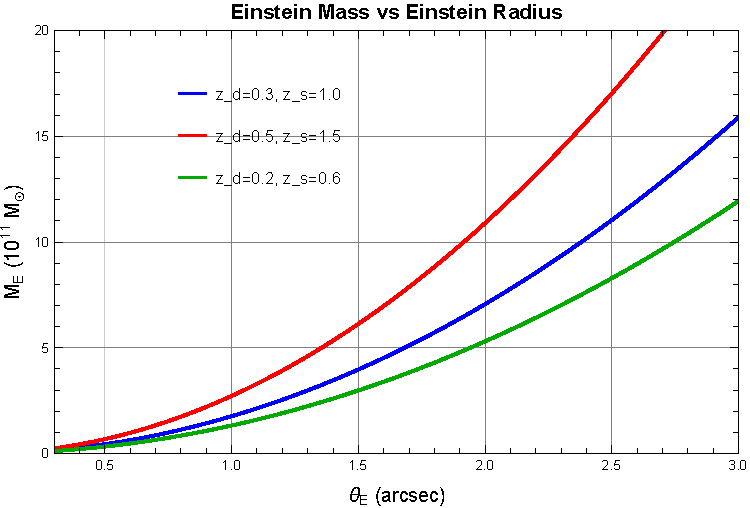
\includegraphics[width=0.75\textwidth]{../Figures/09_Galaxy_Lensing_Applications/einstein_mass_vs_radius.pdf}
    \caption{Enclosed Einstein mass $M_{\mathrm{E}}$ as a function of
    Einstein radius $\thetaE$ for three lens--source redshift
    configurations (flat $\Lambda$CDM, $\Hubble = 70$~km/s/Mpc,
    $\Omegam = 0.3$).  Higher redshift lenses enclose more mass for
    the same angular Einstein radius.
    Generated by \texttt{galaxy\_lensing.wl}.}
    \label{fig:einstein_mass}
\end{figure}

Table~\ref{tab:lens_masses} lists the Einstein radii and enclosed
masses for several well-known lens systems:

\begin{table}[ht]
\centering
\begin{tabular}{lccccc}
\toprule
\textbf{System} & $z_d$ & $z_s$ & $\thetaE$ (arcsec) &
$M_{\mathrm{E}}$ ($10^{11}\,\Msun$) & \textbf{Type} \\
\midrule
Q0957+561  & 0.36 & 1.41 & 1.0  & $\sim 1.9$ & Double \\
Q2237+0305 & 0.04 & 1.69 & 0.9  & $\sim 0.2$ & Quad \\
B1608+656  & 0.63 & 1.39 & 1.0  & $\sim 3.9$ & Quad \\
\bottomrule
\end{tabular}
\caption{Einstein radii and enclosed masses for three well-known
lens systems.  Masses computed using
eq.~\eqref{eq:mass_from_thetaE} with a flat $\Lambda$CDM
cosmology ($\Hubble = 70$~km/s/Mpc, $\Omegam = 0.3$).
Computed by \texttt{galaxy\_lensing.wl}.}
\label{tab:lens_masses}
\end{table}

\begin{remark}
Q2237+0305 (the Einstein Cross) has an unusually small enclosed
mass because the lens galaxy is very nearby ($z_d = 0.04$), so the
physical Einstein radius is small even though the angular Einstein
radius is nearly $1''$.
\end{remark}


% =====================================================================
\section{The Mass-Sheet Degeneracy}
\label{sec:msd}

The \textbf{mass-sheet degeneracy} (MSD) is the most important
systematic limitation of strong gravitational lensing.  It is a
fundamental degeneracy that cannot be broken by lensing data alone
(image positions, flux ratios, or arc morphology).

\subsection{The Mass-Sheet Transform}

Consider a lens with convergence $\kappab(\vectheta)$.  The
\textbf{mass-sheet transform} (MST) replaces this convergence with:
\begin{equation}
    \boxed{
    \kappab_\lambda(\vectheta) = \lambda\,\kappab(\vectheta)
    + (1 - \lambda)
    }
    \label{eq:mst_kappa}
\end{equation}
and simultaneously rescales the source plane:
\begin{equation}
    \boxed{
    \vecbeta_\lambda = \lambda\,\vecbeta
    }
    \label{eq:mst_beta}
\end{equation}
where $\lambda$ is a free parameter.

\begin{annotation}[What $\lambda$ means, and what is invariant]
$1-\lambda$ is the convergence of the added sheet.  $\lambda < 1$ is a positive
sheet (e.g.\ $\lambda = 1-\kappa_{\mathrm{ext}}$ with $\kappa_{\mathrm{ext}} > 0$);
$\lambda > 1$ is a negative sheet, such as an underdense line of sight.
Under the transform:
\begin{itemize}[nosep]
  \item \emph{invariant}: image positions; flux ratios; the critical curves
        ($\Amat_\lambda = \lambda\Amat$ vanishes where $\Amat$ does); the
        Einstein radius (since $\bar\kappab_\lambda = \lambda\bar\kappab + 1 - \lambda = 1$
        iff $\bar\kappab = 1$); and the reduced shear
        $g = \gammaL/(1-\kappab)$, because $\gammaL_\lambda = \lambda\gammaL$
        and $1-\kappab_\lambda = \lambda(1-\kappab)$;
  \item \emph{changed}: $\kappab$ and $\gammaL$ individually, absolute
        magnifications ($\times\lambda^{-2}$), time delays ($\times\lambda$),
        the source size and position ($\times\lambda$), the caustics
        ($\times\lambda$), and the mass profile, whose slope is flattened for
        $\lambda < 1$.
\end{itemize}
Classic error: ``$\thetaE$ is invariant, so the mass inside $\thetaE$ is the
galaxy's mass.''  $M(<\thetaE)$ is indeed invariant, but it includes the sheet:
the \emph{galaxy's} share is $\lambda$ times the original model's.
\end{annotation}


Physically, the MST adds a \textbf{uniform sheet of convergence}
$(1 - \lambda)$ to the lens (hence the name ``mass sheet'') and
rescales both the original convergence and the source plane by
$\lambda$.

\subsection{Image Positions Are Invariant}

The key property of the MST is that it \textbf{preserves all image
positions}.  To see this, recall the lens equation
$\vecbeta = \vectheta - \vecalpha(\vectheta)$.  For the original
lens, the deflection angle is related to the convergence via
$\nabla \cdot \vecalpha = 2\kappab$.  Under the MST:
\begin{equation}
    \vecalpha_\lambda(\vectheta) = \lambda\,\vecalpha(\vectheta)
    + (1 - \lambda)\,\vectheta \,.
    \label{eq:mst_alpha}
\end{equation}
The new lens equation becomes:
\begin{align}
    \vecbeta_\lambda
    &= \vectheta - \vecalpha_\lambda(\vectheta) \notag \\
    &= \vectheta - \lambda\,\vecalpha(\vectheta)
       - (1 - \lambda)\,\vectheta \notag \\
    &= \lambda\,[\vectheta - \vecalpha(\vectheta)] \notag \\
    &= \lambda\,\vecbeta \,.
    \label{eq:mst_lens_eq}
\end{align}
So if $\vectheta$ satisfies the original lens equation for source
position $\vecbeta$, it also satisfies the transformed lens
equation for source position $\vecbeta_\lambda = \lambda\vecbeta$.
\textbf{The image positions are unchanged.}

\begin{derivation}[Where eq.~\eqref{eq:mst_alpha} comes from, and why $\vecbeta \to \lambda\vecbeta$ is forced]
\textit{Potential.}  A uniform sheet of convergence 1 has
$\psiL = |\vectheta|^2/2$: $\nabla\psiL = \vectheta$ and
$\nabla^2\psiL = 2 = 2\kappab$.  So the transformed lens has
\[
  \psiL_\lambda = \lambda\psiL + (1-\lambda)\frac{|\vectheta|^2}{2},
  \qquad
  \nabla^2\psiL_\lambda = \lambda\,2\kappab + 2(1-\lambda) = 2\kappab_\lambda,
  \qquad
  \vecalpha_\lambda = \nabla\psiL_\lambda = \lambda\vecalpha + (1-\lambda)\vectheta .
\]
(The potential is fixed only up to a harmonic function; choosing none is
what makes this the MST, and not a more general transformation.)

\textit{Why the source must rescale.}  The sheet's deflection
$(1-\lambda)\vectheta$ is linear in $\vectheta$, so
$\vectheta - \vecalpha_\lambda = \lambda(\vectheta - \vecalpha)$ holds pointwise.
If $\vectheta_A$ and $\vectheta_B$ are images of $\vecbeta$ in the original
model, both map to the \emph{same} point $\lambda\vecbeta$ in the new one:
they are still images of a single source.  The source position is not
observed, so moving it costs nothing.  This is the whole degeneracy.
\end{derivation}


\subsection{What the MST Changes}

Although image positions are preserved, the MST changes other
observables:

\paragraph{Magnifications.}
Under the MST the transformed convergence and deflection are
\begin{equation*}
    \kappab_\lambda(\vectheta) = \lambda\,\kappab(\vectheta) + (1-\lambda),
    \qquad
    \vecalpha_\lambda(\vectheta) = \lambda\,\vecalpha(\vectheta) + (1-\lambda)\,\vectheta,
\end{equation*}
the second of which follows from the first via
$\vecalpha = \nabla\psiL$ and $\nabla^2\psiL = 2\kappab$
(the $(1-\lambda)\vectheta$ piece is the deflection of a uniform
mass sheet, $\nabla\cdot(\vectheta/2) = 1 = 1 - \lambda$ up to the
overall factor).  The Jacobian then transforms componentwise:
\begin{equation*}
    (\Amat_\lambda)_{ij}
    \;=\; \delta_{ij} - \frac{\partial\alpha_{\lambda,i}}{\partial\theta_j}
    \;=\; \delta_{ij} - \lambda\,\frac{\partial\alpha_i}{\partial\theta_j} - (1-\lambda)\,\delta_{ij}
    \;=\; \lambda\!\left(\delta_{ij} - \frac{\partial\alpha_i}{\partial\theta_j}\right)
    \;=\; \lambda\,\Amat_{ij} \,.
\end{equation*}
That is, every entry of $\Amat$ scales by $\lambda$:
\begin{equation}
    \Amat_\lambda = \lambda\,\Amat,
    \qquad
    \det \Amat_\lambda = \lambda^2\,\det\Amat,
    \label{eq:mst_jacobian}
\end{equation}
so the magnification $\mu = 1/\det\Amat$ scales as
\begin{equation}
    \boxed{
    \mu_\lambda = \frac{1}{\lambda^2}\,\mu \,.}
    \label{eq:mst_magnification}
\end{equation}
Individual magnifications change, but \textbf{magnification ratios}
$\mu_i/\mu_j = \mu_{\lambda,i}/\mu_{\lambda,j}$ are preserved.
This means flux \textit{ratios} cannot distinguish between the
original model and the MST-transformed model.  Both steps are
verified symbolically in
\mathlink{09_Galaxy_Lensing_Applications/galaxy\_lensing.wl}{galaxy\_lensing.wl}.

\begin{annotation}[Reading the parenthesis about $\nabla\cdot(\vectheta/2)$]
The parenthesis above is compressed.  The clean statement is that a sheet of
convergence $\kappab_s$ has deflection $\kappab_s\vectheta$, because
$\nabla\cdot(\kappab_s\vectheta) = 2\kappab_s$ in two dimensions.  With
$\kappab_s = 1-\lambda$ this is the extra term $(1-\lambda)\vectheta$ (previous
box).  A useful corollary: the MST maps the critical curves onto themselves
and shrinks the caustics by $\lambda$, so the \emph{topology} of the image
configuration is unchanged as well.
\end{annotation}


\paragraph{Time delays.}
The Fermat-potential difference between images, and therefore the
model-predicted time delay for a given $\Hubble$, scales as:
\begin{equation}
    \boxed{
    \Delta t_\lambda = \lambda\,\Delta t
    }
    \label{eq:mst_time_delay}
\end{equation}
That is, an MST-transformed model with parameter $\lambda$ produces a
time delay $\lambda$ times that of the original ($\lambda = 1$) model at
the same $\Hubble$.  But the observed $\Delta t$ is fixed; to match
that observation under the transformed model, the inferred
$\Hubble^{\mathrm{naive}}$ that one computes from a $\lambda = 1$
(no-sheet) fit and the underlying ``true'' $\Hubble^{\mathrm{true}}$
that accounts for an actual sheet of parameter $\lambda$ differ by:
\begin{equation}
    \boxed{
    \Hubble^{\mathrm{true}} \;=\; \lambda\,\Hubble^{\mathrm{naive}}
    \quad\Longleftrightarrow\quad
    \Hubble^{\mathrm{naive}} \;=\; \Hubble^{\mathrm{true}} / \lambda \,.
    }
    \label{eq:mst_H0}
\end{equation}
With an unmodeled positive mass sheet ($\lambda < 1$), the naive
analysis therefore \emph{overestimates} $\Hubble$, and including the
sheet brings the inferred value \emph{downward}.  This is the direction
in which TDCOSMO has explored \citep{Birrer2020}: relaxing the lens
profile (equivalently, allowing $\lambda < 1$) shifts the time-delay
$\Hubble$ from the H0LiCOW value
$\Hubble \approx 73.3$~km\,s$^{-1}$\,Mpc$^{-1}$ toward the Planck CMB
value $\Hubble \approx 67.4$~km\,s$^{-1}$\,Mpc$^{-1}$.

\begin{derivation}[Time delays scale by $\lambda$; the sign of the $\Hubble$ correction]
\textit{Fermat potential.}  With
$\tau(\vectheta;\vecbeta) = \tfrac12|\vectheta-\vecbeta|^2 - \psiL(\vectheta)$,
substitute $\vecbeta \to \lambda\vecbeta$ and $\psiL \to \psiL_\lambda$:
\begin{align*}
  \tau_\lambda
  &= \tfrac12|\vectheta|^2 - \lambda\,\vectheta\cdot\vecbeta + \tfrac12\lambda^2|\vecbeta|^2
     - \lambda\psiL - \tfrac12(1-\lambda)|\vectheta|^2\\
  &= \lambda\Big[\tfrac12|\vectheta|^2 - \vectheta\cdot\vecbeta - \psiL\Big] + \tfrac12\lambda^2|\vecbeta|^2\\
  &= \lambda\,\tau(\vectheta;\vecbeta) + \tfrac12\lambda(\lambda-1)|\vecbeta|^2 .
\end{align*}
The last term is the same for every image of the source, so it cancels in
differences: $\Delta\tau_\lambda = \lambda\,\Delta\tau$, which is
eq.~\eqref{eq:mst_time_delay}.

\textit{$\Hubble$.}  The observed delay is fixed:
$\Delta t_{\mathrm{obs}} = D_{\Delta t}(\Hubble)\,\Delta\tau/\speedoflight$
with $D_{\Delta t} \propto 1/\Hubble$, so the inferred
$\Hubble \propto \Delta\tau/\Delta t_{\mathrm{obs}}$.  The naive
($\lambda = 1$) model uses $\Delta\tau$; the true model (its MST) has
$\lambda\Delta\tau$.  Hence
\[
  \frac{\Hubble^{\mathrm{true}}}{\Hubble^{\mathrm{naive}}}
  = \frac{\lambda\,\Delta\tau}{\Delta\tau} = \lambda
  \quad\Longrightarrow\quad
  \Hubble^{\mathrm{true}} = \lambda\,\Hubble^{\mathrm{naive}},
\]
the sign of eq.~\eqref{eq:mst_H0}.  To move $73.3$ to $67.4$ requires
$\lambda = 67.4/73.3 = 0.920$, i.e.\ a sheet of $\kappab_s \approx 0.08$.
\end{derivation}

\begin{annotation}[Sign trap]
Keep three statements together.  (i)~At fixed $\Hubble$ the model delay scales
as $\lambda$.  (ii)~At fixed \emph{observed} delay the inferred $\Hubble$
therefore scales as $\lambda$ too, $\Hubble^{\mathrm{true}} =
\lambda\Hubble^{\mathrm{naive}}$; it does not go as $1/\lambda$.  (iii)~A
positive sheet means $\lambda < 1$, which lowers $\Hubble$.  A one-line
physical check: the transformed model predicts \emph{shorter} delays at fixed
$\Hubble$ ($\lambda\Delta\tau$).  To reproduce the fixed observed delay it
needs a \emph{longer} time-delay distance, $D_{\Delta t} \propto 1/\Hubble$
larger by $1/\lambda$, i.e.\ a smaller $\Hubble$.  If you find yourself
writing $1/\lambda$, recheck which delay is being held fixed.
\end{annotation}


\begin{remark}
The MSD is devastating for time-delay cosmography.  If we model a
lens and infer $\Hubble$ from the time delay, the answer is
degenerate with $\lambda$: any extra convergence (a true mass sheet, or
unmodeled line-of-sight structure, or a profile that is steeper than
assumed) reduces $\Hubble^{\mathrm{true}}$ below
$\Hubble^{\mathrm{naive}}$.  Breaking this degeneracy is the central
challenge of modern time-delay cosmography.
\end{remark}

\begin{annotation}[Steeper or shallower?]
The MST with $\lambda < 1$ makes the profile locally \emph{shallower}.  For
$\kappab \propto \theta^{-s}$, the transformed profile has
\[
  \frac{d\ln\kappab_\lambda}{d\ln\theta}
  = -s\,\frac{\lambda\kappab}{\lambda\kappab + 1 - \lambda},
\]
whose magnitude is smaller than $s$ whenever $0 < \lambda < 1$ and
$\kappab > 0$.  Example: an SIS at $\thetaE$ ($\kappab = 1/2$, $s = 1$) with
$\lambda = 0.9$ has a local slope of $-0.82$ instead of $-1$.  So the pair
``naive model / true model'' related by $\lambda < 1$ is ``steeper / shallower''.
When reading statements about which profile change raises or lowers
$\Hubble$, translate them into $\lambda$ first.
\citet{schneider_sluse_2013} discuss how this degeneracy interacts with the
assumption of a power-law profile in $\Hubble$ inferences.
\end{annotation}


\subsection{Physical Interpretation}

The mass-sheet transform can be interpreted in two ways:
\begin{enumerate}
    \item \textbf{Literal mass sheet:} A uniform sheet of matter
          between the observer and the source (or at the lens
          redshift) adds convergence without changing image positions.
          In practice, line-of-sight structure (voids, filaments,
          galaxy groups along the line of sight) acts as an
          approximate mass sheet.
    \item \textbf{Profile degeneracy:} Even without an actual mass
          sheet, the MST reflects the fact that different radial mass
          profiles can produce the same image positions.  Steeper
          profiles can mimic shallower profiles plus a mass sheet.
\end{enumerate}

Figure~\ref{fig:msd} illustrates the mass-sheet degeneracy: the
left panel shows how the convergence profile changes for different
$\lambda$, and the right panel shows how absolute magnifications
scale as $1/\lambda^2$.

\begin{figure}[ht]
    \centering
    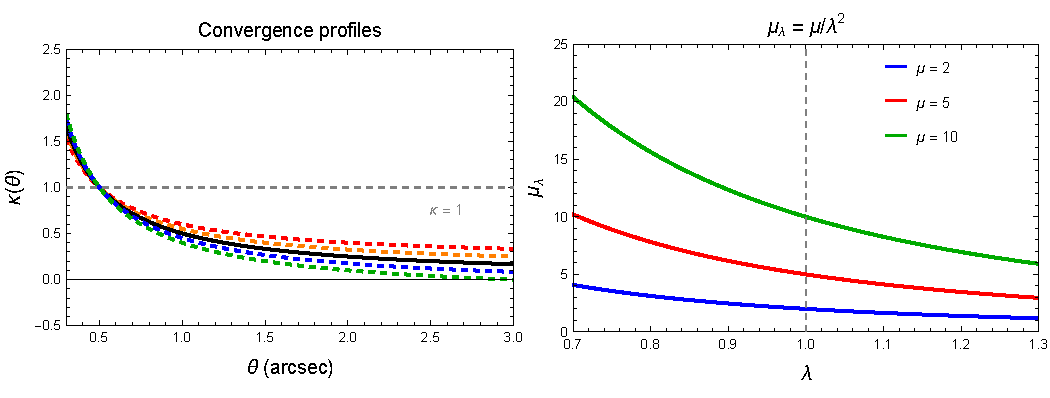
\includegraphics[width=0.85\textwidth]{../Figures/09_Galaxy_Lensing_Applications/mass_sheet_degeneracy.pdf}
    \caption{The mass-sheet degeneracy.  \textbf{Left:}~Convergence
    profiles for an SIS lens ($\thetaE = 1''$) under the MST with
    different $\lambda$ values.  The solid curve is the original
    profile ($\lambda = 1$); dashed curves show the transformed
    profiles.  Curves with $\lambda > 1$ correspond to a negative sheet,
    e.g.\ an underdense line of sight ($\kappa_{\mathrm{ext}} < 0$ in
    $\lambda = 1 - \kappa_{\mathrm{ext}}$).  \textbf{Right:}~Magnification scaling
    $\mu_\lambda = \mu/\lambda^2$ for three different original
    magnifications.
    Generated by \texttt{galaxy\_lensing.wl}.}
    \label{fig:msd}
\end{figure}

\subsection{How to Break the MSD}

Several methods can break or constrain the mass-sheet degeneracy:
\begin{enumerate}
    \item \textbf{Stellar kinematics:} The velocity dispersion
          $\sigma_v$ of the lens galaxy depends on the mass profile
          slope, not just the enclosed mass.  A mass-sheet transform
          changes the predicted $\sigma_v$, so a kinematic measurement
          constrains $\lambda$ (Section~\ref{sec:lensing_kinematics}).
    \item \textbf{Standardizable magnifications:} If the source has a
          known intrinsic luminosity (e.g., a Type Ia supernova),
          the absolute magnification can be measured, breaking the
          MSD.
    \item \textbf{Multiple source planes:} If the same lens produces
          images of sources at different redshifts, the different
          $\Sigmacr$ values for each source plane break the
          degeneracy.
    \item \textbf{Extended source reconstruction:} Detailed modeling
          of extended arcs constrains the lens potential more tightly,
          partially breaking the degeneracy (though not completely).
\end{enumerate}

\begin{bridge}[Chapter~\ref{ch:msd_kinematics}: the MST with two source planes]
Item~3 needs care.  Take one deflector and two sources, ignoring the mass of
the first source: $\vecbeta_i = \vectheta - \eta_i\vecalpha(\vectheta)$, with
$\eta_1 = 1$ and $\eta_2 = \eta < 1$ a distance ratio.  Apply the MST of plane~1
to the physical deflector.  Plane~2 then sees
$\vectheta - \eta[\lambda\vecalpha + (1-\lambda)\vectheta]$, which can be
rewritten exactly as
\[
  c\,\big(\vectheta - \eta'\vecalpha\big),
  \qquad c = 1 - \eta(1-\lambda),
  \qquad \eta' = \frac{\lambda\eta}{c},
\]
with $\eta' - \eta = \eta(1-\eta)(\lambda-1)/c$.  So the images of
\emph{both} planes are preserved provided the distance ratio is changed from
$\eta$ to $\eta'$ (and source~2 rescaled by $c$).  If cosmology fixes $\eta$,
only $\lambda = 1$ survives: the second plane breaks the MST.  If $\eta$ is a
free parameter, which is the case when one wants to \emph{measure} cosmology
from a DSPL, the MST survives as a $\lambda$--$\eta$ degeneracy.
Chapter~\ref{ch:msd_kinematics} develops this and shows how the lens-galaxy
velocity dispersion, which responds to the physical mass inside the aperture,
can pin $\lambda$ down.
\end{bridge}



% =====================================================================
\section{The Source Position Transformation}
\label{sec:spt}

The mass-sheet degeneracy is a special case of a more general class
of transformations that preserve image positions.

\subsection{Definition}

The \textbf{source position transformation} (SPT), introduced by
Schneider \& Sluse (2014), is any invertible mapping of the source
plane:
\begin{equation}
    \vecbeta \to \hat{\vecbeta}(\vecbeta)
    \label{eq:spt_def}
\end{equation}
that, when combined with a suitably modified lens equation, preserves
all image positions.  The modified lens equation is:
\begin{equation}
    \hat{\vecbeta}(\vecbeta)
    = \vectheta - \hat{\vecalpha}(\vectheta)
    \label{eq:spt_lens_eq}
\end{equation}
where the new deflection field $\hat{\vecalpha}$ is defined by the
requirement that all observed image positions map to the transformed
source position $\hat{\vecbeta}$.

The MST is the special case where $\hat{\vecbeta} = \lambda\vecbeta$
(a linear scaling).  The SPT generalizes this to arbitrary nonlinear
remappings of the source plane.

\begin{derivation}[What an SPT does to the Jacobian, and why most SPTs are only approximate]
Define the new deflection by
$\hat{\vecalpha}(\vectheta) \equiv \vectheta - \hat{\vecbeta}\big(\vecbeta(\vectheta)\big)$,
so that eq.~\eqref{eq:spt_lens_eq} holds by construction and every image of
$\vecbeta$ maps to $\hat{\vecbeta}(\vecbeta)$.  Then, by the chain rule,
\[
  \hat{\Amat}(\vectheta) \equiv \frac{\partial\hat{\vecbeta}}{\partial\vectheta}
  = \mathcal{B}\big(\vecbeta(\vectheta)\big)\,\Amat(\vectheta),
  \qquad \mathcal{B} \equiv \frac{\partial\hat{\vecbeta}}{\partial\vecbeta}.
\]
\begin{enumerate}[nosep]
  \item \textit{Flux ratios.}  $\hat\mu = 1/\det(\mathcal{B}\Amat) =
        \mu/\det\mathcal{B}$.  All images of one source share the same
        $\vecbeta$, hence the same $\det\mathcal{B}$, so ratios are preserved.
  \item \textit{Is $\hat{\vecalpha}$ a deflection?}  A lens deflection is a
        gradient, so $\hat\Amat$ must be symmetric.  For the MST,
        $\mathcal{B} = \lambda\mathbb{I}$ and $\lambda\Amat$ is symmetric.  For
        a general $\mathcal{B}$, $\mathcal{B}\Amat$ is symmetric only if
        $\mathcal{B}$ and $\Amat$ commute, which fails generically (e.g.\
        $\mathcal{B} = \begin{pmatrix}1.1&0.05\\0.05&0.95\end{pmatrix}$,
        $\Amat = \begin{pmatrix}0.4&0.2\\0.2&-0.3\end{pmatrix}$ give an
        asymmetric product).
\end{enumerate}
Hence a generic SPT does not correspond exactly to any mass distribution.
It does only approximately, over the region where the images lie, which is
why \citet{schneider_sluse_2014} call it an approximate invariance.  The MST
is the exact member of the family.
\end{derivation}


\subsection{Implications}

The SPT is an active area of research because it defines the
\textit{full} class of degeneracies in strong lensing.  Key results
include:
\begin{itemize}
    \item Not all SPTs correspond to physically valid lens models
          (i.e., the transformed deflection field may not come from a
          non-negative mass distribution).
    \item The SPT preserves image positions and flux \textit{ratios}
          (just as the MST does) but generically changes absolute
          magnifications and time delays.
    \item Breaking the SPT generally requires external information
          (kinematics, multiple source planes, or standardizable
          sources), just as for the MST.
\end{itemize}

\begin{remark}
The SPT shows that the mass-sheet degeneracy is not a peculiarity of
a specific transform but rather the simplest member of a broad family
of degeneracies inherent in the lensing inverse problem.  Any attempt
to measure $\Hubble$ from time delays must confront this fundamental
limitation.
\end{remark}


% =====================================================================
\section{Strong Lensing and Stellar Kinematics}
\label{sec:lensing_kinematics}

Combining strong lensing with stellar kinematics is one of the most
powerful approaches to studying galaxy mass distributions.  The two
techniques are complementary in a fundamental way.

\subsection{What Each Technique Measures}

\paragraph{Strong lensing:}
Measures the \textbf{total projected mass} (dark matter + stars +
gas) within the Einstein radius $\thetaE$.  The measurement is
model-independent for a circularly symmetric lens
(eq.~\ref{eq:mass_from_thetaE}).  For an elliptical model, the
enclosed mass depends weakly on the assumed axis ratio but is still
robust.

\paragraph{Stellar kinematics:}
The stellar velocity dispersion $\sigma_v$ of the lens galaxy,
measured from absorption line broadening, probes the gravitational
potential.  Specifically, under the assumption of dynamical
equilibrium (the Jeans equation), the luminosity-weighted line-of-sight
velocity dispersion within an aperture $R_{\mathrm{ap}}$ depends on:
\begin{itemize}[nosep]
    \item The \textbf{mass profile slope} (how mass is distributed
          radially).
    \item The \textbf{total mass normalization}.
    \item The \textbf{orbital anisotropy} of the stellar orbits.
\end{itemize}

\subsection{The Power-Law Mass Profile}
\label{sec:power_law_profile}

The simplest model that captures the essential physics is a
\textbf{spherical power-law} density profile:
\begin{equation}
    \boxed{
    \rho(r) = \rho_0 \left(\frac{r}{r_0}\right)^{-\gamma'}
    }
    \label{eq:power_law_rho}
\end{equation}
where $\gamma'$ is the power-law slope.  The isothermal case is
$\gamma' = 2$ (i.e., $\rho \propto r^{-2}$).

Figure~\ref{fig:power_law} shows convergence profiles and enclosed
mass scalings for power-law density profiles with different slopes.

\begin{figure}[ht]
    \centering
    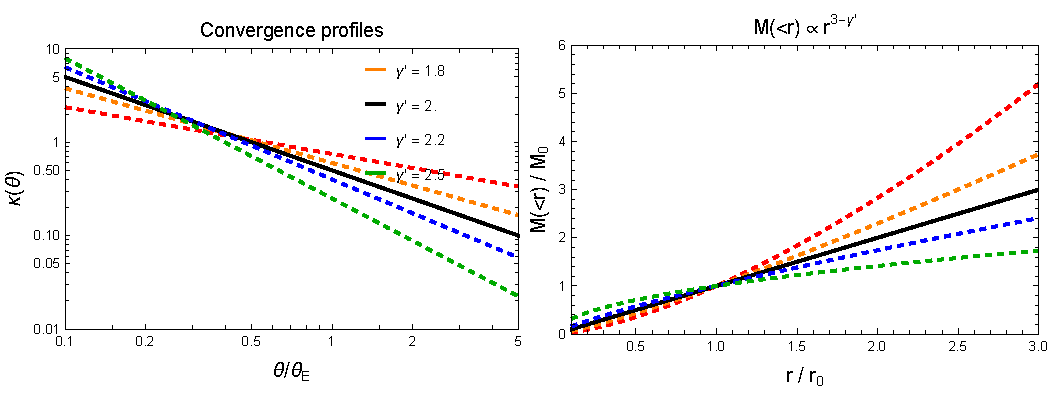
\includegraphics[width=0.85\textwidth]{../Figures/09_Galaxy_Lensing_Applications/power_law_profiles.pdf}
    \caption{Power-law density profiles $\rho \propto r^{-\gamma'}$.
    \textbf{Left:}~Convergence profiles for different slopes (the
    solid curve is the isothermal case $\gamma' = 2$).
    \textbf{Right:}~Enclosed 3D mass $M(\le r) \propto
    r^{3-\gamma'}$ for the same slopes.
    Generated by \texttt{galaxy\_lensing.wl}.}
    \label{fig:power_law}
\end{figure}

The convergence follows from the line-of-sight projection.  Writing
$r = \sqrt{\xi^2 + z^2}$,
\begin{equation*}
    \Sigma(\xi) \;=\; \int_{-\infty}^{\infty}\!
        \rho_0\!\left(\frac{\sqrt{\xi^2+z^2}}{r_0}\right)^{\!-\gamma'}\!\!dz
    \;=\; 2\rho_0\,r_0^{\gamma'}\,\xi^{1-\gamma'}\!
        \int_0^{\infty}\!(1+u^2)^{-\gamma'/2}\,du
    \qquad (u = z/\xi).
\end{equation*}
The remaining integral is a Beta function:
\begin{equation*}
    \int_0^{\infty}(1 + u^2)^{-\gamma'/2}\,du
    \;=\; \frac{1}{2}\,B\!\left(\frac{1}{2},\frac{\gamma'-1}{2}\right)
    \;=\; \frac{\sqrt{\pi}}{2}\,
        \frac{\Gamma\!\left(\frac{\gamma'-1}{2}\right)}{\Gamma\!\left(\frac{\gamma'}{2}\right)},
\end{equation*}
finite for $\gamma' > 1$.  Hence $\Sigma(\xi) \propto \xi^{1-\gamma'}$
and, using $\xi = \Dd\theta$ and dividing by $\Sigmacr$, the
convergence has the same exponent.  A short computation that fixes
the overall normalization by matching to the isothermal case
$\gamma' = 2$ (where $\thetaE$ is the SIS Einstein radius) gives
\begin{equation}
    \kappab(\theta) \;=\; \frac{3 - \gamma'}{2}\,
        \left(\frac{\thetaE}{\theta}\right)^{\!\gamma' - 1},
    \label{eq:kappa_power_law}
\end{equation}
valid for $1 < \gamma' < 3$ (finite projection, finite enclosed
mass).  The projection integral and the normalization are verified
in \texttt{galaxy\_lensing.wl}.
and the Einstein radius is:
\begin{equation}
    \thetaE = 4\pi\,\frac{\sigma_{\mathrm{SIE}}^2}{\speedoflight^2}
    \,\frac{\Dds}{\Ds}\,f(\gamma')
    \label{eq:thetaE_power_law}
\end{equation}
where $f(\gamma')$ is a function of the slope that equals unity for
$\gamma' = 2$ (recovering the SIE result) and $\sigma_{\mathrm{SIE}}$
is the SIE-equivalent velocity dispersion.

\begin{derivation}[Projection of $\rho \propto r^{-\gamma'}$ and the normalization of eq.~\eqref{eq:kappa_power_law}]
\textit{Projection.}  Put $z = \xi u$, $dz = \xi\,du$:
\[
  \rho_0 r_0^{\gamma'}(\xi^2 + z^2)^{-\gamma'/2}dz
  = \rho_0 r_0^{\gamma'}\,\xi^{1-\gamma'}(1+u^2)^{-\gamma'/2}du .
\]
Then substitute $t = u^2/(1+u^2)$, which turns the integral into the Beta
integral $\tfrac12\int_0^1 t^{-1/2}(1-t)^{(\gamma'-3)/2}dt =
\tfrac12 B\big(\tfrac12,\tfrac{\gamma'-1}{2}\big)$.  It converges only for
$\gamma' > 1$.  $B(a,b) = \Gamma(a)\Gamma(b)/\Gamma(a+b)$ with
$\Gamma(1/2) = \sqrt\pi$ gives the $\Gamma$-ratio form.  Check:
$\gamma' = 2$ gives $\tfrac{\sqrt\pi}{2}\Gamma(\tfrac12)/\Gamma(1) = \pi/2$,
and $\int_0^\infty du/(1+u^2) = \pi/2$.

\textit{Normalization.}  Write $\kappab = A(\thetaE/\theta)^{\gamma'-1}$.  The
mean convergence inside $\theta$ is
\[
  \bar\kappab(\theta) = \frac{2}{\theta^2}\int_0^\theta\kappab\,\theta'\,d\theta'
  = \frac{2A}{3-\gamma'}\Big(\frac{\thetaE}{\theta}\Big)^{\gamma'-1}
  \qquad (\gamma' < 3).
\]
The Einstein-radius condition $\bar\kappab(\thetaE) = 1$ gives
$A = (3-\gamma')/2$.  The condition actually imposed is ``mean convergence
1 at $\thetaE$''.  ``Matching the isothermal case'' is then the check that
$\gamma' = 2$ returns $\thetaE/(2\theta)$.

\textit{Consequences} (used repeatedly in Part~V):
\begin{itemize}[nosep]
  \item $\kappab(\thetaE) = (3-\gamma')/2$: $1/2$ for isothermal, larger for
        shallower profiles;
  \item $\alpha(\theta) = \theta\bar\kappab = \thetaE^{\gamma'-1}\theta^{2-\gamma'}$;
  \item $M_{\mathrm{2D}}(<\theta) \propto \theta^{3-\gamma'}$;
  \item radial critical curve: $1 - d\alpha/d\theta = 0$ at
        $\theta_r = \thetaE(2-\gamma')^{1/(\gamma'-1)}$, which exists only
        for $\gamma' < 2$.
\end{itemize}
\end{derivation}

\begin{annotation}[Which ``slope''?  $\gamma'$ versus the 2D slope versus $\gammaL$]
$\gamma'$ is the \emph{three-dimensional} density slope.  The projected
convergence falls as $\theta^{1-\gamma'}$, a 2D log-slope of $-(\gamma'-1)$:
$-1$ for isothermal, not $-2$.  The deflection goes as $\theta^{2-\gamma'}$.
The prime is there to avoid confusion with the shear $\gammaL$; papers using
$\gamma$ for the slope must be read carefully.  Classic error: plugging the 2D
slope into a 3D formula, which is off by one.
\end{annotation}

\begin{bridge}[Chapter~\ref{ch:power_law_point_mass}: the projected power law]
Chapter~\ref{ch:power_law_point_mass} adds a central point mass to exactly
this profile.  It needs $\alpha(\theta) = \thetaE^{\gamma'-1}\theta^{2-\gamma'}$
(the point mass simply adds $\theta_\bullet^2/\theta$), the convergence
$(3-\gamma')/2$ at $\thetaE$, and the radial critical curve
$\theta_r = \thetaE(2-\gamma')^{1/(\gamma'-1)}$, which exists only for
$\gamma' < 2$.  Whether a radial critical curve exists, and where, controls
the central image that a point mass can perturb or suppress.
\end{bridge}


\subsection{Breaking the Degeneracy}

The key insight is that lensing and kinematics respond differently to
the mass profile slope $\gamma'$:

\begin{itemize}
    \item \textbf{Lensing} constrains the projected mass within
          $\thetaE$.  For a power-law profile, the enclosed mass
          $M_{\mathrm{E}}$ depends on the normalization $\rho_0$ and
          the slope $\gamma'$ in a specific way.
    \item \textbf{Kinematics} constrains the mass within the
          spectroscopic aperture (typically a different physical
          radius than $R_{\mathrm{E}}$).  The predicted
          $\sigma_v^2$ depends on $\gamma'$ \textit{differently}
          from how $M_{\mathrm{E}}$ does.
\end{itemize}

By measuring both $M_{\mathrm{E}}$ (from lensing) and $\sigma_v$
(from spectroscopy), one can solve for \textit{both} the mass
normalization and the slope $\gamma'$.  This breaks the mass-sheet
degeneracy because the MST changes the effective $\gamma'$:
steepening or shallowing the profile to compensate for the added
mass sheet.

\begin{derivation}[A Jeans-equation sketch: why $\sigma_v$ depends on $\gamma'$]
For a spherical, isotropic, non-rotating tracer of density
$\nu(r) \propto r^{-\delta}$ in a potential with enclosed mass
$M(r) = m_0 r^{3-\gamma'}$, the Jeans equation is
\[
  \frac{d(\nu\sigma_r^2)}{dr} = -\nu\frac{\Gnewton M(r)}{r^2}
  \quad\Longrightarrow\quad
  \nu\sigma_r^2 = \int_r^\infty \nu\,\frac{\Gnewton M}{r'^2}\,dr'
\]
(taking $\nu\sigma_r^2 \to 0$ at infinity).  The integrand scales as
$r'^{1-\gamma'-\delta}$, so for $\gamma' + \delta > 2$
\[
  \sigma_r^2(r) = \frac{\Gnewton M(r)}{r}\,\frac{1}{\gamma' + \delta - 2}
  \;\xrightarrow{\ \delta = \gamma'\ }\;
  \frac{\Gnewton M(r)}{2(\gamma'-1)\,r} .
\]
Checks: $\gamma' = 2$ gives $\sigma_r^2 = \Gnewton M/(2r)$, i.e.\ the SIS
$M(r) = 2\sigma^2r/\Gnewton$; and $\sigma_r^2 \propto r^{2-\gamma'}$ is flat
only for the isothermal slope.  The observable, a luminosity-weighted,
projected, aperture-averaged $\sigma_v$, adds $\gamma'$- and
anisotropy-dependent factors (the $g(\gamma')$ of
Exercise~\ref{ex:power_law_profile}).  The essential point already shows
here: $\sigma_v^2$ measures $M(r)/r$ at the aperture radius, while lensing
fixes $M_{\mathrm{2D}}(<\RE)$.  Two radii, two constraints, so slope and
normalization separate.
\end{derivation}


\subsection{The Bulge-Halo Conspiracy}
\label{sec:conspiracy}

One of the most remarkable results from combining lensing and
kinematics is the \textbf{bulge-halo conspiracy}: the total (dark
matter + stellar) density profiles of massive elliptical galaxies
are remarkably close to isothermal over a wide range of radii:
\begin{equation}
    \gamma' \approx 2.0 \pm 0.2
    \label{eq:conspiracy}
\end{equation}
This result, established by the SLACS survey (Auger et al.\ 2010)
and confirmed by subsequent studies, means that the combined
contribution of the stellar bulge (which has a steeper profile,
$\gamma' \sim 3$) and the dark matter halo (which has a shallower
inner profile, $\gamma' \sim 1$ for NFW) conspire to produce an
approximately $r^{-2}$ total density profile.

Figure~\ref{fig:lensing_kinematics} shows how the predicted
velocity dispersion varies with $\gamma'$ for a fixed Einstein
mass, illustrating how kinematics breaks the degeneracy.

\begin{figure}[ht]
    \centering
    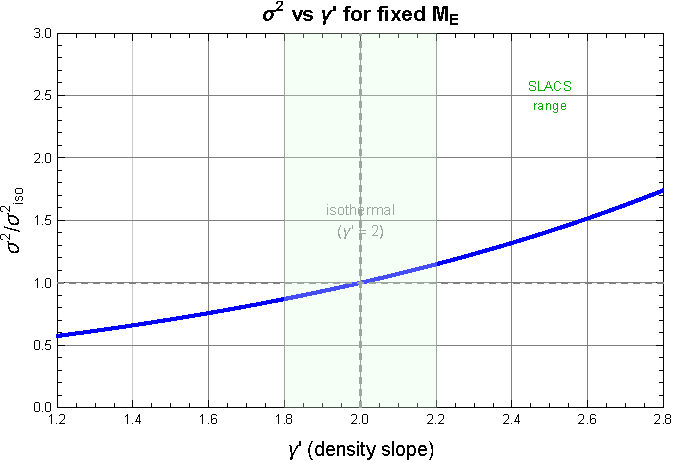
\includegraphics[width=0.65\textwidth]{../Figures/09_Galaxy_Lensing_Applications/lensing_kinematics.pdf}
    \caption{Predicted $\sigma_v^2$ (normalized to the isothermal
    value) as a function of the density slope $\gamma'$, for fixed
    Einstein mass.  The green band shows the range found by the
    SLACS survey ($\gamma' \approx 2.0 \pm 0.2$).  Measuring
    $\sigma_v$ constrains $\gamma'$ and breaks the mass-sheet
    degeneracy.
    Generated by \texttt{galaxy\_lensing.wl}.}
    \label{fig:lensing_kinematics}
\end{figure}

This ``conspiracy'' is not fully understood theoretically and
remains an active area of research.  It has important implications:
\begin{enumerate}
    \item The SIE ($\gamma' = 2$) is a good approximation for most
          galaxy-scale lenses.
    \item The small scatter in $\gamma'$ suggests a universal mass
          assembly process for massive ellipticals.
    \item It connects directly to the flat rotation curves observed
          in spiral galaxies (both are consequences of
          $\rho \propto r^{-2}$).
\end{enumerate}

\begin{bridge}[Chapter~\ref{ch:central_mass_bias}: the slope--central-mass trade is a ``local MST'']
Images near $\thetaE$ constrain, to first order, $\alpha(\thetaE)$ and
$d\alpha/d\theta$ at $\thetaE$.  For an axisymmetric lens with fixed $\thetaE$,
these are equivalent to $\kappab(\thetaE)$.  Now give a power law of slope
$\gamma'$ a central point mass of Einstein radius $\theta_\bullet$, with
$f = \theta_\bullet^2/\thetaE^2$, and renormalize the galaxy so that $\thetaE$
is unchanged.  The composite matches $\alpha$ and $d\alpha/d\theta$ at $\thetaE$
of a \emph{pure} power law with
\[
  \gamma'_{\mathrm{eff}} = \gamma' + f\,(3-\gamma')
\]
(e.g.\ $f = 0.05$, $\gamma' = 2$ gives $2.05$).  An unmodelled central mass
therefore looks like a steeper profile.  This is the MST idea applied over
the annulus of the images rather than globally, and
Chapter~\ref{ch:central_mass_bias} quantifies the bias it induces.
\end{bridge}



% =====================================================================
\section{Time-Delay Cosmography}
\label{sec:time_delay_cosmography}

Strong lens time delays offer a one-step measurement of $\Hubble$,
independent of the cosmic distance ladder.

\subsection{Recap: Time Delays and $\Hubble$}

From Module~\ref{ch:fermat_time_delays}, the time delay between
images $A$ and $B$ of a strongly lensed variable source is:
\begin{equation}
    \Delta t_{AB} = \frac{1 + z_d}{\speedoflight}
    \,\frac{\Dd\,\Ds}{\Dds}
    \,\left[\Delta\tau_{AB}\right]
    \label{eq:time_delay_recap}
\end{equation}
where $\Delta\tau_{AB}$ is the Fermat potential difference (computed
from the lens model) and the prefactor $\Dd\Ds/\Dds$ is called the
\textbf{time-delay distance} $D_{\Delta t}$.  Crucially:
\begin{equation}
    D_{\Delta t} \propto \frac{1}{\Hubble}
    \label{eq:Ddt_H0}
\end{equation}
so measuring $\Delta t$ (from monitoring the variable source) and
modeling $\Delta\tau$ (from the lens model) gives $\Hubble$.

\begin{derivation}[Why $D_{\Delta t} \propto 1/\Hubble$]
In an FRW model every angular-diameter distance has the form
$D_{ij} = (\speedoflight/\Hubble)\,f_{ij}(z_i, z_j; \Omegam, \ldots)$, with
$f_{ij}$ dimensionless.  Then
\[
  \frac{\Dd\Ds}{\Dds}
  = \frac{(\speedoflight/\Hubble)f_d\,(\speedoflight/\Hubble)f_s}{(\speedoflight/\Hubble)f_{ds}}
  = \frac{\speedoflight}{\Hubble}\,\frac{f_df_s}{f_{ds}} .
\]
One power of $\speedoflight/\Hubble$ survives.  Halving $\Hubble$ doubles
$D_{\Delta t}$ (checked numerically for $z_d = 0.6$, $z_s = 1.5$).
\end{derivation}

\begin{annotation}[Two conventions for $D_{\Delta t}$, and a unit check]
Here the prefactor $\Dd\Ds/\Dds$ is called $D_{\Delta t}$ and $(1+z_d)$ is
written separately.  Exercise~\ref{ex:H0_time_delay} and much of the
literature fold it in, $D_{\Delta t} = (1+z_d)\Dd\Ds/\Dds$.  Both are
$\propto 1/\Hubble$; just do not include $(1+z_d)$ twice.  Unit check with the
exercise's numbers: $(1+z_d)\Dd\Ds/\Dds = 4463$~Mpc and
$\Delta\tau = 0.64$~arcsec$^2 = 1.504\times10^{-11}$~rad$^2$ give
$D_{\Delta t}\Delta\tau/\speedoflight = 80.0$~days.  $\Delta\tau$ must be in
rad$^2$.
\end{annotation}

\begin{bridge}[Chapter~\ref{ch:cosmological_sensitivity}: what each distance combination constrains]
$D_{\Delta t}$ carries one power of $\speedoflight/\Hubble$, so time delays
measure $\Hubble$.
Every \emph{ratio} of distances, such as $\Dds/\Ds$, or the DSPL ratio of two
such ratios, is independent of $\Hubble$: the $\speedoflight/\Hubble$ factors
cancel (checked numerically).  A DSPL therefore constrains
the density parameters (and the dark-energy equation of state), not
$\Hubble$.  Chapter~\ref{ch:cosmological_sensitivity}
compares the two sensitivities; the MST affects them differently, since time
delays scale with $\lambda$ while the DSPL ratio is degenerate with $\lambda$
only through the $\eta'$ relation of the bridge in \S\ref{sec:msd}.
\end{bridge}


\subsection{The H0LiCOW / TDCOSMO Program}

The most extensive application of this method is the
\textbf{H0LiCOW} (H0 Lenses in COSMOGRAIL's Wellspring) program
and its successor \textbf{TDCOSMO}, which have analyzed six
well-studied time-delay lenses.

The headline result from Wong et al.\ (2020), assuming power-law
mass profiles:
\begin{equation}
    \boxed{
    \Hubble = 73.3^{+1.7}_{-1.8}
    \;\mathrm{km\,s^{-1}\,Mpc^{-1}}
    }
    \label{eq:H0LiCOW}
\end{equation}
at 2.4\% precision.  This value is in $3.1\sigma$ tension with the
Planck CMB measurement (Planck Collaboration 2020):
\begin{equation}
    \Hubble^{\mathrm{Planck}} = 67.4 \pm 0.5
    \;\mathrm{km\,s^{-1}\,Mpc^{-1}}
    \label{eq:H0_Planck}
\end{equation}
and agrees well with the local distance ladder value from SH0ES
(Riess et al.\ 2022):
\begin{equation}
    \Hubble^{\mathrm{SH0ES}} = 73.0 \pm 1.0
    \;\mathrm{km\,s^{-1}\,Mpc^{-1}} \,.
    \label{eq:H0_SH0ES}
\end{equation}

Figure~\ref{fig:h0_time_delay} illustrates the effect of the
mass-sheet degeneracy on the inferred $\Hubble$.

\begin{figure}[ht]
    \centering
    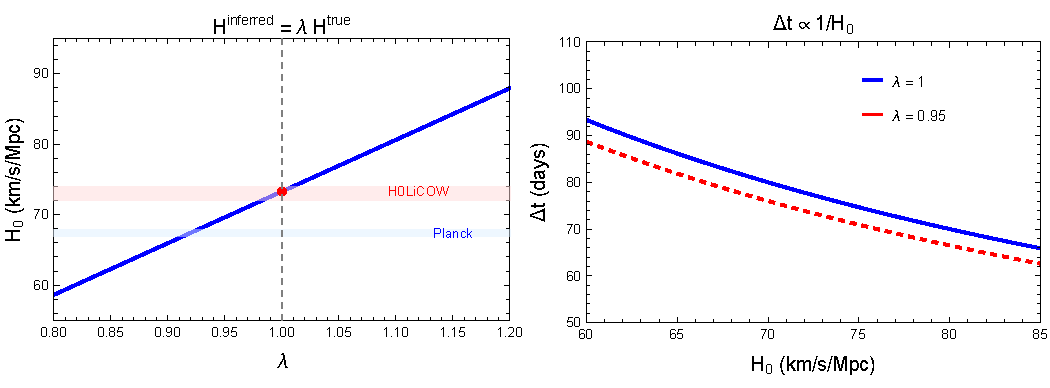
\includegraphics[width=0.85\textwidth]{../Figures/09_Galaxy_Lensing_Applications/h0_time_delay.pdf}
    \caption{Time-delay cosmography and the mass-sheet degeneracy.
    \textbf{Left:}~Inferred $\Hubble$ as a function of the MST
    parameter $\lambda$, showing the H0LiCOW measurement (red
    point) and the Planck and SH0ES bands.
    \textbf{Right:}~Time delay vs.\ $\Hubble$ for $\lambda = 1$
    (solid) and $\lambda = 0.95$ (dashed).
    Generated by \texttt{galaxy\_lensing.wl}.}
    \label{fig:h0_time_delay}
\end{figure}

\subsection{The Role of the Mass-Sheet Degeneracy}

The mass-sheet degeneracy is the dominant systematic uncertainty in
time-delay cosmography.  From eq.~\eqref{eq:mst_H0}:
\begin{equation}
    \Hubble^{\mathrm{true}} = \lambda\,\Hubble^{\mathrm{naive}}
\end{equation}
where $\Hubble^{\mathrm{naive}}$ is the $\Hubble$ inferred from a
no-sheet ($\lambda = 1$) power-law fit and $\Hubble^{\mathrm{true}}$
is the actual cosmological value; since $\lambda < 1$ for an
unmodeled positive mass sheet, $\Hubble^{\mathrm{true}} <
\Hubble^{\mathrm{naive}}$.
A 10\% mass sheet ($\lambda = 0.9$, i.e., adding $\kappab_s = 0.1$
to the convergence) shifts $\Hubble^{\mathrm{naive}}$ downward by 10\%.

\begin{annotation}[What ``shifts downward by 10\%'' means]
Read the last sentence as: with $\lambda = 0.9$ the \emph{true} value is
$0.9\,\Hubble^{\mathrm{naive}}$, 10\% below the naive one.  The naive number
itself is whatever the no-sheet fit returns; the correction moves the
\emph{inference} downward.  Equivalently, the naive value overestimates the
truth by $1/\lambda - 1 = 11\%$.
\end{annotation}


The TDCOSMO collaboration (Birrer et al.\ 2020) showed that relaxing
the assumption of a power-law mass profile (which partially encodes
$\lambda$) broadens the uncertainty to:
\begin{equation}
    \Hubble = 74.5^{+5.6}_{-6.1}
    \;\mathrm{km\,s^{-1}\,Mpc^{-1}}
    \label{eq:TDCOSMO_relaxed}
\end{equation}
--- still consistent with the local value but with much larger
uncertainty.  The increased uncertainty is almost entirely due to
the mass-sheet degeneracy.

Constraining $\lambda$ requires external information, primarily
\textbf{stellar kinematics} of the lens galaxies
(Section~\ref{sec:lensing_kinematics}).

\subsection{Current State and Future Prospects}

The time-delay cosmography method is a key player in the Hubble
tension debate.  Upcoming surveys (Rubin Observatory/LSST, Euclid)
will discover thousands of new lensed quasars, enabling a
statistical approach that can average over individual modeling
uncertainties.  Combined with improved stellar kinematics from
next-generation spectrographs, the method has the potential to
reach $\sim$1\% precision on $\Hubble$.


% =====================================================================
\section{Real Lens Systems: Case Studies}
\label{sec:case_studies}

\subsection{Q0957+561: The First Gravitational Lens}

Discovered by Walsh, Carswell \& Weymann in 1979, Q0957+561 was
the first confirmed strong gravitational lens.  Key properties:
\begin{itemize}[nosep]
    \item \textbf{Configuration:} Double (two images of a $z_s = 1.41$
          quasar).
    \item \textbf{Lens:} Giant elliptical galaxy at $z_d = 0.36$,
          in a galaxy cluster.
    \item \textbf{Einstein radius:} $\thetaE \approx 1.0''$.
    \item \textbf{Time delay:} $\Delta t = 417 \pm 3$ days (optical
          monitoring; Kundi\'c et al.\ 1997; see
          \citealp[][Part~1, p.~12]{schneider_kochanek_wambsganss_2006}).
    \item \textbf{Historical significance:} Confirmation of Einstein's
          prediction of multiple imaging by galaxies.  The long time
          delay was the first used for $\Hubble$ estimation (Refsdal's
          method).
\end{itemize}

\subsection{Q2237+0305: The Einstein Cross}

Q2237+0305 is one of the most photogenic gravitational lenses:
\begin{itemize}[nosep]
    \item \textbf{Configuration:} Quad --- four images of a
          $z_s = 1.69$ quasar arranged in a near-perfect Einstein
          cross around the nucleus of a nearby barred spiral galaxy.
    \item \textbf{Lens:} A face-on barred spiral galaxy at
          $z_d = 0.04$ (Huchra's Lens).  This is the nearest known
          strong lens galaxy.
    \item \textbf{Einstein radius:} $\thetaE \approx 0.9''$.
    \item \textbf{Special feature:} Because the lens is so nearby,
          the Einstein radius corresponds to a very small physical
          radius ($\sim 0.7$~kpc), probing deep into the bulge of
          the spiral galaxy.  The system shows dramatic
          \textbf{microlensing} variability as individual stars in
          the lens galaxy cross the lines of sight to the quasar
          images.
    \item \textbf{Time delays:} Very short ($\lesssim 1$ day) due
          to the symmetric geometry, making this system unsuitable
          for $\Hubble$ measurement but ideal for microlensing
          studies.
\end{itemize}

\subsection{B1608+656: Time-Delay Cosmography}

B1608+656 is one of the best-studied time-delay lenses:
\begin{itemize}[nosep]
    \item \textbf{Configuration:} Quad --- four images of a
          $z_s = 1.39$ radio source.
    \item \textbf{Lens:} Two interacting galaxies at $z_d = 0.63$.
    \item \textbf{Einstein radius:} $\thetaE \approx 1.0''$.
    \item \textbf{Time delays:} Three independent delays measured
          with $\sim$1--2\% precision from radio monitoring.
    \item \textbf{Cosmographic result:} One of the six TDCOSMO/H0LiCOW
          lenses used to constrain $\Hubble$.  The lens modeling is
          more complex than usual due to the two-galaxy lens
          configuration.
    \item \textbf{Key insight:} Deep HST imaging resolves the
          lensed host galaxy of the radio source, providing extended
          arc constraints that significantly tighten the lens model.
\end{itemize}


% =====================================================================
\section{Substructure and Flux-Ratio Anomalies}
\label{sec:substructure}

Everything so far has treated the lens as a \emph{smooth} mass
distribution.  But $\Lambda$CDM predicts that galaxy haloes are lumpy:
$N$-body simulations produce far more low-mass subhaloes than the number
of luminous satellites we observe (the ``missing satellites'' problem),
with of order a few percent of the projected mass near the images bound
in substructure \citep[][Part~2, \S8]{schneider_kochanek_wambsganss_2006}.
Strong lensing offers a way to weigh this \emph{dark} substructure.

\subsection{The Flux-Ratio Anomaly}
\label{sec:flux_anomaly}

Lens models that fit the image \emph{positions} of a quad to
milliarcsecond precision routinely fail to reproduce the image
\emph{flux ratios}.  For a source straddling a fold or cusp of the
caustic, smooth models make sharp predictions --- e.g.\ the
\textbf{cusp relation}, that the signed magnifications of the three
merging images of a cusp image sum to zero --- and real systems (the
classic case is the radio quad B1422$+$231) violate them.  Optical flux
ratios can be corrupted by microlensing (Module~\ref{ch:microlensing})
and dust; but \emph{radio} flux ratios are largely immune to both, and
they are anomalous just the same.

\subsection{Why Flux Ratios Probe Low-Mass Substructure}
\label{sec:why_flux}

The key is how many derivatives of the potential each observable
requires.  For virialized objects $M \propto \sigma_v^4$ and
$R \propto \sigma_v^2$, so:
\begin{itemize}[nosep]
    \item \textbf{time delays} $\propto \psiL \propto M \propto \sigma_v^4$
          --- unaffected by low-mass substructure;
    \item \textbf{deflections} $\propto \nabla\psiL \propto \sigma_v^2$
          --- perturbed only by \emph{massive} substructure;
    \item \textbf{magnifications} $\kappab,\gammaL \propto \nabla^2\psiL
          \propto \sigma_v^0$ --- perturbed \emph{equally by all mass
          scales}.
\end{itemize}
Flux ratios (magnifications) are therefore uniquely sensitive to the
low-mass end of the substructure spectrum, exactly where CDM and warm
dark matter differ.  A further diagnostic is that substructure
preferentially \emph{demagnifies saddle-point} images relative to minima
\citep[][Part~2, \S8]{schneider_kochanek_wambsganss_2006}.  Applying a
Bayesian analysis to a sample of radio quads, Dalal \& Kochanek found a
substructure mass fraction $f_{\mathrm{sat}} \approx 0.02$ (90\%
confidence $0.006$--$0.07$), consistent with CDM and far above the
luminous-satellite fraction.  Modern work extends this with
\textbf{gravitational imaging} --- detecting individual dark subhaloes
through their astrometric perturbations of extended arcs --- turning
flux-ratio and arc anomalies into a probe of the small-scale matter
power spectrum.


% =====================================================================
\section{Extended Sources and Einstein-Ring Reconstruction}
\label{sec:extended_sources}

Real sources are extended, and their lensed images --- arcs and
\textbf{Einstein rings} --- carry far more information than a handful of
point images.  The foundational fact is that
\textbf{gravitational lensing conserves surface brightness}:
\begin{equation}
    f_I(\vectheta) = f_S(\vecbeta(\vectheta)),
    \label{eq:sb_conservation}
\end{equation}
so what we call ``magnification'' is only the apparent brightening that
follows from the image subtending a larger solid angle than the source;
the intrinsic surface brightness is unchanged
\citep[][Part~2, \S10]{schneider_kochanek_wambsganss_2006}.

\subsection{The Einstein Ring as a Pattern}
\label{sec:ring_pattern}

An Einstein ring is not a set of discrete images but a \emph{pattern}:
the locus of peak surface brightness along radial spokes from the lens
centre.  For an isothermal lens with arbitrary angular structure,
$\psiL = b\,\theta\,F(\varphi)$ with $\langle F\rangle = 1$, the
tangential critical curve sits at
\begin{equation}
    \frac{r_{\mathrm{crit}}}{b} = F(\varphi) + F''(\varphi),
    \label{eq:ring_crit}
\end{equation}
while, for a compact source offset by $\vecbeta_0$ from the lens centre,
the ring curve is
\begin{equation}
    \frac{r_E(\varphi)}{b} = F(\varphi) + \vecbeta_0 \cdot \hat{e}_\theta
    \label{eq:ring_curve}
\end{equation}
\citep[Kochanek, Keeton \& McLeod 2001; see][Part~2, eq.~141]{schneider_kochanek_wambsganss_2006}.
The remarkable consequence is that the \emph{angular shape} of the ring
directly reads off the multipoles $F(\varphi)$ of the lens potential
(\S\ref{sec:multipoles} of Module~\ref{ch:elliptical_models}): the even
multipoles of the ring encode the lens, the odd multipoles the source.
Rings thus break the angular degeneracies that a two-image lens cannot
constrain --- though they pin down the \emph{radial} profile only weakly
(the dependence scales as $|\Delta\beta|^4$).

\subsection{Source Reconstruction}
\label{sec:source_reconstruction}

To use every pixel of an arc, one reconstructs the source.  Because
surface brightness is conserved, every image-plane pixel maps to a source
position $\vecbeta(\vectheta,\mathbf{p})$ for lens parameters
$\mathbf{p}$; in a \emph{correct} model all image pixels mapping to the
same source pixel share a surface brightness, while an incorrect model
scatters them.  Minimizing that scatter --- the ``Ring Cycle'' idea,
now realized as regularized linear (semilinear) inversion onto a pixel
or adaptive grid --- underlies modern pipelines such as
\texttt{PyAutoLens} and the SLaM framework used in surveys like AGEL.
This is the practical engine behind galaxy-scale mass measurements and
the source-plane reconstructions of high-redshift galaxies.


% =====================================================================
\section{External Convergence and Lens Environments}
\label{sec:external_convergence}

No lens is isolated.  Mass in the lens's group or cluster, and
uncorrelated structure along the line of sight, contribute an
\textbf{external convergence} $\kappa_{\mathrm{ext}}$ that is nearly
uniform across the image region --- i.e.\ a mass sheet.  As we saw in
\S\ref{sec:msd}, a uniform sheet leaves the image positions and flux
ratios unchanged (it is the physical realization of the mass-sheet
transform with $\lambda = 1 - \kappa_{\mathrm{ext}}$), but it rescales an
inferred Hubble constant,
\begin{equation}
    \Hubble^{\mathrm{true}}
    = (1 - \kappa_{\mathrm{ext}})\,\Hubble^{\mathrm{naive}},
    \label{eq:kappa_ext_H0}
\end{equation}
exactly as in Eq.~\eqref{eq:mst_H0}.  Estimating
$\kappa_{\mathrm{ext}}$ --- typically a few percent --- from the
photometric and spectroscopic weighting of the lens field, calibrated
against numerical line-of-sight simulations, is an essential and
irreducible step in time-delay cosmography
\citep{wong_h0licow_2020,Birrer2020}.

\begin{annotation}[Scale of the effect]
Since $\Hubble^{\mathrm{true}} = (1-\kappa_{\mathrm{ext}})\Hubble^{\mathrm{naive}}$,
an error $\delta\kappa_{\mathrm{ext}}$ maps one-to-one onto a fractional error
in $\Hubble$.  Each 0.01 in $\kappa_{\mathrm{ext}}$ is a 1\% shift, which is
why a 2\% $\Hubble$ requires $\kappa_{\mathrm{ext}}$ to about 0.02 or better
per lens (or averaged over many lenses).  For scale, closing the whole
73.3-versus-67.4 gap with a sheet alone would need
$\kappa_{\mathrm{ext}} \approx 0.08$.
\end{annotation}


\subsection{Dust and the Interstellar Medium of the Lens}
\label{sec:lens_dust}

A more mundane environmental effect is the \textbf{interstellar medium of
the lens galaxy}.  Differential extinction reddens and dims the optical
and near-infrared images that pass through different lines of sight in
the lens, corrupting optical flux ratios (and biasing colours) in a
strongly wavelength-dependent way
\citep[][Part~2, \S9]{schneider_kochanek_wambsganss_2006}.  This is a
principal reason the substructure studies of \S\ref{sec:substructure}
rely on \emph{radio} flux ratios, which are essentially dust-free, and a
reminder that a clean lensing measurement must always account for the
baryonic astrophysics of the deflector.


% =====================================================================
\section{Summary}
\label{sec:galaxy_lensing_summary}

\begin{itemize}
    \item The \textbf{Einstein radius} provides a model-independent
          measurement of the enclosed projected mass:
          $M_{\mathrm{E}} = \pi\thetaE^2 \Dd^2 \Sigmacr$.  For
          typical galaxy-scale lenses, this mass is
          $10^{11}$--$10^{12}\,\Msun$.

    \item The standard parametric lens model is \textbf{SIE +
          external shear}, with 7 parameters.  Quad lenses provide
          8 positional constraints, marginally determining the model.

    \item The \textbf{mass-sheet degeneracy} (MST:
          $\kappab \to \lambda\kappab + (1-\lambda)$,
          $\vecbeta \to \lambda\vecbeta$) preserves all image
          positions but changes magnifications by $1/\lambda^2$ and
          time delays by $\lambda$.  It is the dominant systematic
          for time-delay cosmography.

    \item The \textbf{source position transformation} (Schneider \&
          Sluse 2014) generalizes the MST to arbitrary remappings
          $\vecbeta \to \hat{\vecbeta}(\vecbeta)$ of the source
          plane.

    \item \textbf{Lensing + kinematics} breaks the MSD by
          constraining the density profile slope $\gamma'$.  The
          SLACS survey found $\gamma' \approx 2.0 \pm 0.2$ (the
          ``bulge-halo conspiracy'').

    \item \textbf{Time-delay cosmography} measures $\Hubble$ via
          $\Delta t \propto D_{\Delta t} \propto 1/\Hubble$.  The
          H0LiCOW/TDCOSMO result is $\Hubble = 73.3^{+1.7}_{-1.8}$
          km/s/Mpc, in tension with Planck.

    \item \textbf{Case studies:} Q0957+561 (first lens, 1979),
          Q2237+0305 (Einstein Cross, microlensing laboratory),
          B1608+656 (time-delay cosmography).
\end{itemize}


% =====================================================================
\section{Problems}
\label{sec:galaxy_lensing_problems}

\begin{exercise}
\label{ex:sie_mass}
\textbf{(Enclosed mass for an SIE lens.)}
Consider an SIE lens with $\thetaE = 1.5''$, axis ratio $q = 0.8$,
lens redshift $z_d = 0.3$, and source redshift $z_s = 1.0$.
Assume a flat $\Lambda$CDM cosmology with $\Hubble = 70$~km/s/Mpc
and $\Omegam = 0.3$.
\begin{enumerate}[label=(\alph*)]
    \item Compute the angular diameter distances $\Dd$, $\Ds$, and
          $\Dds$.
    \item Compute the critical surface mass density $\Sigmacr$.
    \item Compute the enclosed projected mass $M_{\mathrm{E}}$ using
          eq.~\eqref{eq:mass_from_thetaE}.  Express the result in
          solar masses.
    \item Estimate the velocity dispersion $\sigma_v$ that would
          correspond to this Einstein radius using
          eq.~\eqref{eq:thetaE_sie}.
\end{enumerate}
Verify with
\solnlink{09_Galaxy_Lensing_Applications/problems\_09.wl}{problems\_09.wl}.
\end{exercise}

\begin{exercise}
\label{ex:msd_derivation}
\textbf{(Mass-sheet degeneracy: invariance and observables.)}
Consider a general lens with convergence $\kappab(\vectheta)$ and a
source at $\vecbeta$.
\begin{enumerate}[label=(\alph*)]
    \item Apply the mass-sheet transform
          $\kappab_\lambda = \lambda\kappab + (1-\lambda)$ and
          $\vecbeta_\lambda = \lambda\vecbeta$.  Show explicitly that
          the lens equation
          $\vecbeta_\lambda = \vectheta -
          \vecalpha_\lambda(\vectheta)$ is satisfied at the same image
          positions $\vectheta$.
    \item Show that the Jacobian matrix transforms as
          $\Amat_\lambda = \lambda\,\Amat$ and hence the
          magnification transforms as
          $\mu_\lambda = \mu/\lambda^2$.
    \item Show that magnification \textit{ratios}
          $\mu_i/\mu_j$ are invariant under the MST.
    \item Using the Fermat potential, show that time delays
          transform as $\Delta t_\lambda = \lambda\,\Delta t$.
\end{enumerate}
Verify with
\solnlink{09_Galaxy_Lensing_Applications/problems\_09.wl}{problems\_09.wl}.
\end{exercise}

\begin{exercise}
\label{ex:H0_time_delay}
\textbf{($\Hubble$ from a time-delay lens.)}
A quad lens at $z_d = 0.6$, $z_s = 1.5$ has a measured time delay
$\Delta t = 80$ days between two images.  The lens model predicts
a Fermat potential difference $\Delta\tau = 0.64$~arcsec$^2$.
\begin{enumerate}[label=(\alph*)]
    \item Write the time-delay equation
          (eq.~\ref{eq:time_delay_recap}) and solve for $\Hubble$.
    \item Compute $\Hubble$ numerically, assuming a flat $\Lambda$CDM
          cosmology with $\Omegam = 0.3$ and using the angular
          diameter distances at the given redshifts.  \textit{(Hint:
          the time-delay distance $D_{\Delta t} = (1+z_d)\Dd\Ds/\Dds$
          depends on $\Hubble$, so you will need to solve
          self-consistently or use $\Hubble$-independent distance
          ratios.)}
    \item Discuss: if the true lens includes a mass sheet with
          $\kappab_s = 0.05$ (i.e., $\lambda = 0.95$) that was not
          accounted for in the model, how would the inferred $\Hubble$
          change?
\end{enumerate}
Verify with
\solnlink{09_Galaxy_Lensing_Applications/problems\_09.wl}{problems\_09.wl}.
\end{exercise}

\begin{exercise}
\label{ex:power_law_profile}
\textbf{(Power-law profile: lensing and kinematics.)}
Consider a spherical power-law density profile
$\rho(r) = \rho_0 (r/r_0)^{-\gamma'}$.
\begin{enumerate}[label=(\alph*)]
    \item Compute the projected surface mass density
          $\Sigma(\theta)$ by integrating $\rho$ along the line of
          sight.  Show that
          $\kappab(\theta) \propto \theta^{1-\gamma'}$.
    \item For $\gamma' = 2$ (isothermal), verify that you recover
          $\kappab \propto 1/\theta$ (the SIS).
    \item The luminosity-weighted line-of-sight velocity dispersion
          for an isotropic power-law profile is (Treu \& Koopmans
          2004):
          \[
              \sigma_v^2 \propto M(\le R_{\mathrm{ap}}) \cdot
              R_{\mathrm{ap}}^{-1} \cdot g(\gamma')
          \]
          where $g(\gamma')$ is a known function of the slope.
          Argue that $\sigma_v$ depends on $\gamma'$ differently
          from $M_{\mathrm{E}}$, so combining the two measurements
          constrains $\gamma'$.
    \item For a lens with $\thetaE = 1.2''$ and
          $\sigma_v = 230$~km/s, compute $\gamma'$ assuming the
          relation holds.  Discuss whether the result is consistent
          with the ``bulge-halo conspiracy''
          ($\gamma' \approx 2.0$).
\end{enumerate}
Verify with
\solnlink{09_Galaxy_Lensing_Applications/problems\_09.wl}{problems\_09.wl}.
\end{exercise}

\begin{exercise}
\label{ex:compare_lenses}
\textbf{(Comparing real lens systems.)}
Consider the three lens systems in Table~\ref{tab:lens_masses}:
Q0957+561 ($z_d = 0.36$, $z_s = 1.41$, $\thetaE = 1.0''$),
Q2237+0305 ($z_d = 0.04$, $z_s = 1.69$, $\thetaE = 0.9''$), and
B1608+656 ($z_d = 0.63$, $z_s = 1.39$, $\thetaE = 1.0''$).
\begin{enumerate}[label=(\alph*)]
    \item For each system, compute the angular diameter distances
          $\Dd$, $\Ds$, $\Dds$ and the critical surface mass
          density $\Sigmacr$.
    \item Compute the enclosed projected mass $M_{\mathrm{E}}$ for
          each system.
    \item Compute the physical Einstein radius $R_{\mathrm{E}} =
          \Dd\,\thetaE$ in kpc for each system.
    \item Which system has the largest enclosed mass?  Which has the
          largest physical Einstein radius?  Discuss why the rankings
          are different.
\end{enumerate}
Verify with
\solnlink{09_Galaxy_Lensing_Applications/problems\_09.wl}{problems\_09.wl}.
\end{exercise}
